\section{結果}\label{sec:results}
本章では，報酬設計1（ゴール到達報酬のみ）および
報酬設計2（ステップ負報酬＋壁衝突ペナルティ）における
学習曲線の比較結果を示す．図中のエラーバーは
複数試行（runs=5）におけるばらつきを表す．
以降のPRQにおける方策選択（バンディット）手法は，
事前のグリッドサーチにより各条件で良好であったパラメータを用いた．
具体的には，報酬設計1では 
Boltzmann（$\tau_0=0.0,\, d\tau=0.05$），
$\varepsilon$-greedy（$\varepsilon_b=0.05$），
UCB（$c=0.3$），
報酬設計2では Boltzmann（$\tau_0=0.05,\, d\tau=0.05$），
$\varepsilon$-greedy（$\varepsilon_b=0.2$），
UCB（$c=0.1$）を用いた．
なお，Baseline は$\varepsilon$-greedy による
通常のQ学習である．

\subsection{報酬設計1（ゴール到達報酬のみ）の結果}
報酬設計1においては，いずれのタスクにおいても 
PRQ（方策再利用）系列が Baseline を一貫して上回り，
学習初期から累積平均利得（cumulative mean gain）
がより大きくなる傾向が確認できる．
例えば Task 1（goal=(2,2)）では，3手法はいずれも
 Baseline より高い利得を示し，
 特にUCBが終盤までわずかに高い値を維持した．
 一方で Boltzmann と$\varepsilon$-greedy は
 近い性能で推移し，差は小さい（図1相当）．

Task 5（goal=(12,12)）では，$\varepsilon$-greedy が
学習初期から立ち上がりが速く，終盤まで高い利得を示した．
ただし，$\varepsilon$-greedy はエラーバーが比較的大きく，
試行間のばらつきが大きいことも確認できる．UCBは他2手法より
やや低い曲線となった（図2相当）．

Task 12（goal=(9,1)）および Task 15（goal=(21,5)）では，
UCBとBoltzmannが高い性能を示し，$\varepsilon$-greedy は
それらに比べて明確に低い利得で推移した．特にTask 15では，
UCBが学習初期から大きく優位であり，Boltzmannがそれに続き，
$\varepsilon$-greedy は中盤以降に改善するものの差が残った
（図3，図4相当）．
以上より，報酬設計1では PRQ により Baseline を大きく上回る改善が
得られ，その中でもタスクによって最も有効な方策選択手法が
変化することが示唆される
（例：Task 5では$\varepsilon$-greedyが優位，
Task 12/15ではUCBやBoltzmannが優位）．

\subsection{報酬設計2（ステップ負報酬＋壁衝突ペナルティ）の結果}
報酬設計2では，ステップ負報酬および壁衝突ペナルティの導入により，
累積平均利得が全体として負の領域から推移するタスクが多く見られた．
しかしその場合でも，PRQ系列は Baseline より一貫して
高い値（より負が小さい，あるいは0に近い）を示し，
報酬設計を変更しても方策再利用が学習効率改善に寄与することが
確認できる．

Task 1（goal=(2,2)）では，3手法の曲線はほぼ重なって推移し，
方策選択手法間の差は小さい一方，PRQ系列は 
Baseline を大きく上回った（図5相当）．
Task 5（goal=(12,12)）では，Boltzmannが最も高い利得を示し，
$\varepsilon$-greedy がそれに続いた．
UCBは他2手法より低い曲線となり，
特に終盤で差が残った．

Task 9（goal=(15,19)）および Task 12（goal=(9,1)）では，
UCBが全体として最も高い利得を示し，Boltzmannがそれに続き，
$\varepsilon$-greedy が相対的に低い傾向となった（図7，図8相当）．
このように報酬設計2では，報酬のスケールや負報酬の影響により
曲線の絶対値は変化するものの，PRQ系列の優位性自体は維持され，
さらにタスクによってはUCBが安定して高い性能を示す一方，
Task 5のようにBoltzmannが優位となるケースも確認された．

% --- ここから図（4枚） ---
\begin{figure}[!b]
  \centering
  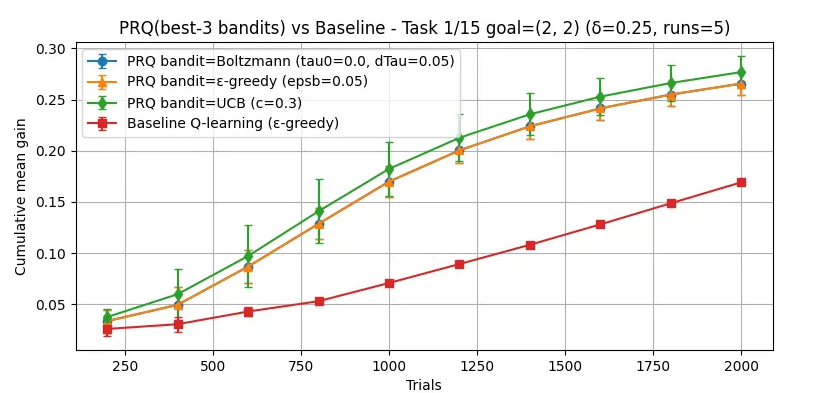
\includegraphics[width=0.90\columnwidth]{../contents/figure/reward1_task01.png}
  \caption{報酬設計1における学習曲線（Task 1）}
  \label{fig:r1_task1}
\end{figure}

\vspace{-1.0em}
\begin{figure}[!b]
  \centering
  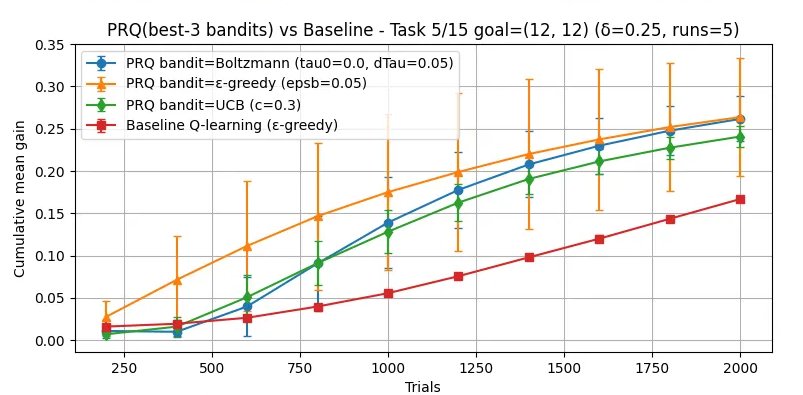
\includegraphics[width=0.90\columnwidth]{../contents/figure/reward1_task05.png}
  \caption{報酬設計1における学習曲線（Task 5）}
  \label{fig:r1_task5}
\end{figure}

\vspace{-1.0em}
\begin{figure}[!b]
  \centering
  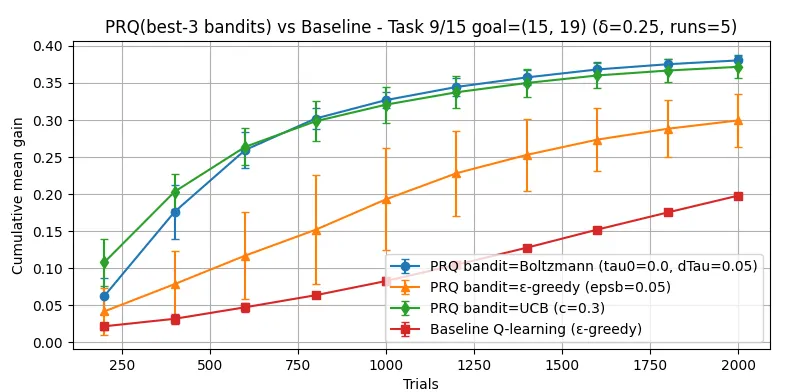
\includegraphics[width=0.90\columnwidth]{../contents/figure/reward1_task09.png}
  \caption{報酬設計1における学習曲線（Task 9）}
  \label{fig:r1_task9}
\end{figure}

\vspace{-1.0em}
\begin{figure}[!b]
  \centering
  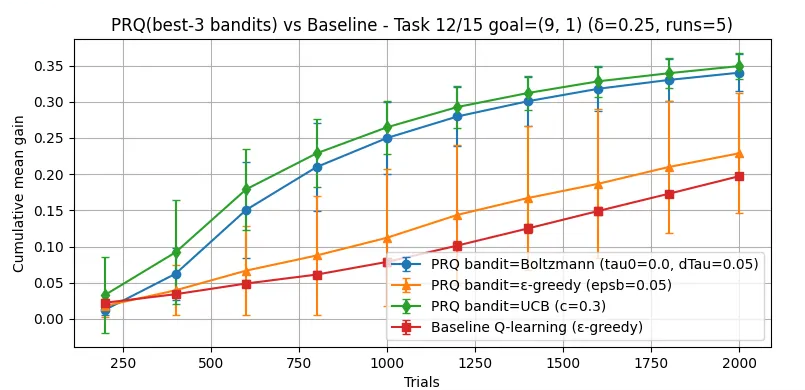
\includegraphics[width=0.90\columnwidth]{../contents/figure/reward1_task12.png}
  \caption{報酬設計1における学習曲線（Task 12）}
  \label{fig:r1_task12}
\end{figure}

%-----ここから６枚

% （前提）プリアンブルに入れておく：
% \usepackage{float}

% 次ページ（次スライド）頭から開始
\clearpage

% --- 残り6枚：左上から縦に並べる（固定配置） ---

\begin{figure}[H]
  \centering
  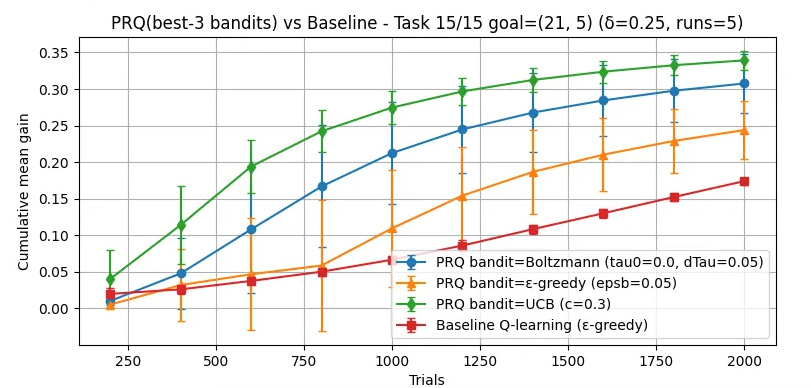
\includegraphics[width=0.90\columnwidth]{../contents/figure/reward1_task15.png}
  \caption{報酬設計1：Task 15}
  \label{fig:r1_task15}
\end{figure}

\vspace{-0.8em}
\begin{figure}[H]
  \centering
  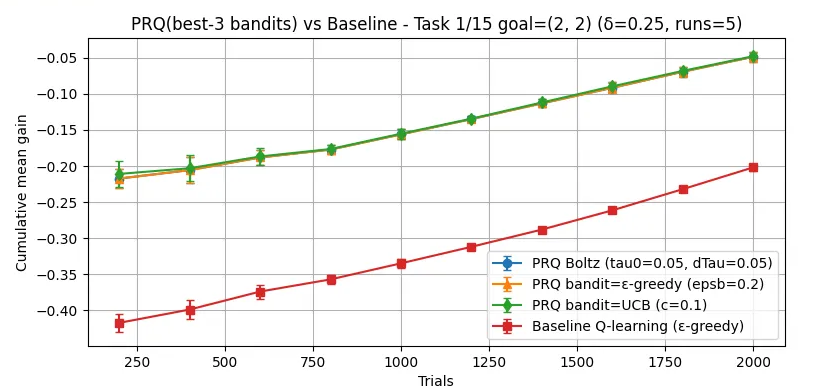
\includegraphics[width=0.90\columnwidth]{../contents/figure/reward2_task01.png}
  \caption{報酬設計2：Task 1}
  \label{fig:r2_task1}
\end{figure}

\vspace{-0.8em}
\begin{figure}[H]
  \centering
  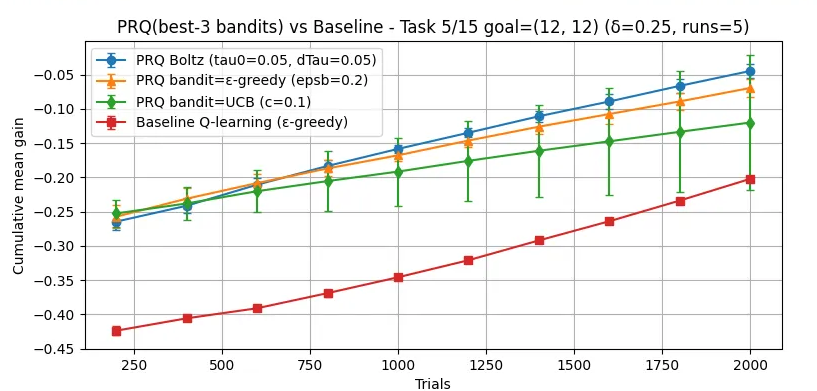
\includegraphics[width=0.90\columnwidth]{../contents/figure/reward2_task05.png}
  \caption{報酬設計2：Task 5}
  \label{fig:r2_task5}
\end{figure}

\vspace{-0.8em}
\begin{figure}[H]
  \centering
  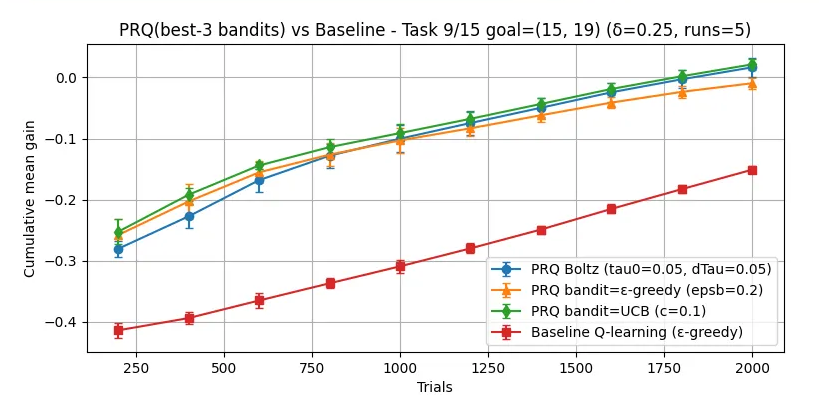
\includegraphics[width=0.90\columnwidth]{../contents/figure/reward2_task09.png}
  \caption{報酬設計2：Task 9}
  \label{fig:r2_task9}
\end{figure}

\vspace{-0.8em}
\begin{figure}[H]
  \centering
  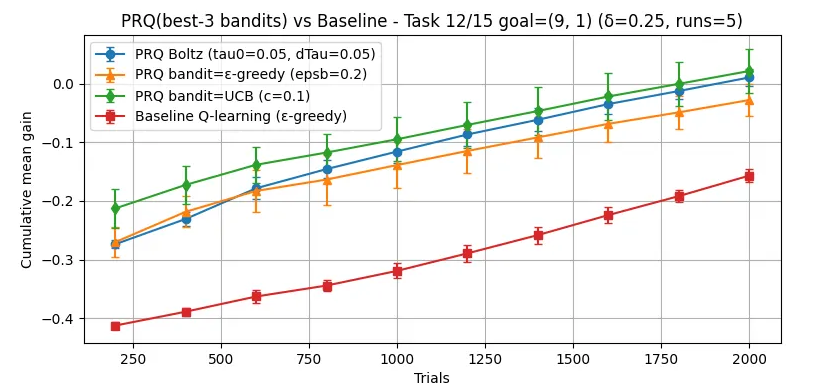
\includegraphics[width=0.90\columnwidth]{../contents/figure/reward2_task12.png}
  \caption{報酬設計2：Task 12}
  \label{fig:r2_task12}
\end{figure}

\vspace{-0.8em}
\begin{figure}[H]
  \centering
  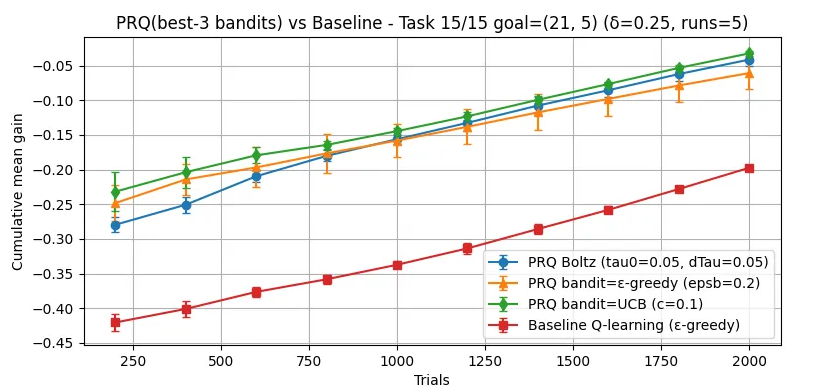
\includegraphics[width=0.90\columnwidth]{../contents/figure/reward2_task15.png}
  \caption{報酬設計2：Task 15}
  \label{fig:r2_task15}
\end{figure}
